\chapter{Analýza existujících řešení}

\setcounter{page}{1}

\begin{chapterabstract}
V rámci této kapitoly provádím rešerši podobných řešení s cílem zjistit jejich funkčnosti a UI.
\end{chapterabstract}

\section{politiscope}

\begin{description}
	\item \textbf{Autor:} Android Politiscope Developer
	\item \textbf{Počet stažení:} více než 10 000
	\item \textbf{Analyzovaná verze:} 2.4 (26. 1., 2023)
\end{description}

Aplikace politiscope \cite{politiscope} dle popisu na Google Play poskytuje informace ohledně politiky ve Spojených Státech v zjednodušené formě. Aplikace poskytuje informace i politicích a jejich rozhodnutích v hlasováních. Informace jsou podávány jednodušší formou, přičemž se snaží udržet objektivitu podaných informací. Aktuální témata jsou barevně označena pro lepší UX. Uživatelé mají možnost uložit si návrh zákona a sledovat průběh hlasování. Uživatelé mají také možnost sledovat konkrétní politiky. Návrhy zákonů jsou označeny tagy pro snazší vyhledání. U témat jsou i oficiální sumarizace a odkazy na oficiální zdroje. Lze také sledovat průběh voleb a kampaně.

Aplikace čerpá data z API poskytuných z následujícíh portálů:

\begin{itemize}
	\item https://api.propublica.org/ - ProPublica je nezávislá, nezisková redakce. \cite{propublica}
	\item https://theunitedstates.io/ - @unitedstates je projekt poskytující data ohledně Spojených Států veřejností a pro veřejnost. \cite{unitedstates}
	\item https://www.congress.gov/ - Congress.gov je oficiální portál pro informace z Kongresu a orgánů státní správy. \cite{congress}
	\item https://api.open.fec.gov/ - OpenFEC je oficiální portál vlády Spojených Států. \cite{openfec}
\end{itemize}

Výše uvedené informace jsou čerpány čistě z popisu a screenshotů aplikace na Google Playi. Do aplikace se mi nepodařilo dostat. Pro přístup je potřeba se zaregistrovat a přihlásit se. Při registraci mě to však automaticky přesměruje na obrazovka pro přihlášování. Při zadání přihlašovacích údaju to však píše, že účet se zadanými přihlašovacími údaji neexistují. Aplikaci jsem testoval na dvou různých zařízeních a na obou nastal ten samý problém. Aplikace má přesto přes 10 000 stažení, a tudíž ve většině případech funguje. Tipuji, že problém souvisí s geografickou lokací mobilního zařízení.

\begin{figure}
	\centering

	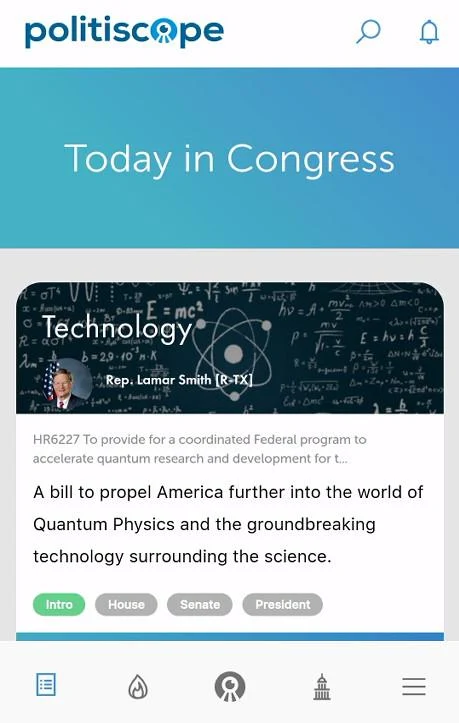
\includegraphics[width=0.4\linewidth]{politiscope}
	
\includegraphics[width=0.4\linewidth]{politiscope2}
	
	\caption{Android aplikace politiscope}
	\label{fig:politoscope}
\end{figure}

\subsection{Zhodnocení}
Přestože aplikaci se mi nepodařilo zprovoznit, stálo za podle mého názoru ji sem dát kvůli jejímu rozsáhlému výčtu funkčností. Další výhodou této aplikace je také přívětivé uživatelské rozhraní a fakt, že data získává z API. Poslanecká sněmovna, jak později ukážu, API pro svoje data neposkytuje, ale data poskytuje ve formě CSV souborů.

\section{Congress}

\begin{description}
	\item \textbf{Autor:} Eric Mill
	\item \textbf{Počet stažení:} více než 500 000
	\item \textbf{Analyzovaná verze:} 4.9.2 (27. 1., 2023)
\end{description}

Aplikace Congress \cite{congress} dle popisu na Google Play poskytuje informace ohledně politických reprezentantů a jejich hlasováních, a návrhů zákonů ve Spojených Státech. Návrhy a hlasování umožňuje vyhledávat.

Při spuštění aplikace uvidíme domovskou obrazovku, která obsahuje menu pro seznam politiků, návrhů zákonů, výsledků hlasování, aktivity v kongresu, schůzky komisí a seznam komisí. Na domovské stránce uvidíme také seznam nejnovějších návrhů zákonů. 

Obrazovka pro seznam politiků obsahuje seznam politiků, které aktuálně sledujeme, seznam politických reprezentantů rozdělených podle států, sněmovny a senátu. Na obrazovce konkrétního politického reprezentanta uvidíme jméno, politickou stranu, příslušný stát, telefonní číslo, jak hlasoval, které zákony navrhnul, ke kterým komisím přísluší, odkaz na oficiální stránku s informacemi o něm a jeho biografii. 

Obrazovka pro návrhy zákonů obsahuje seznam návrhů, které sledujeme, seznam aktivních návrhů a seznam nových návrhů.

Na obrazovce pro výsledky hlasování je popis, výsledek datum a čas, a údaj o tomm, zda se hlasovalo ve Sněmovně nebo Senátu. Obrazovka s detailem hlasování obsahuje výsledek hlasování, počet hlasování pro a proti, a počet lidí, kteří nehlasovali. Dále obsahuje informace o tom, kolik lidí je potřeba být ve fyzické přítomnosti, aby hlasování bylo platné, a jak hlasoval který politik.

Obrazovka pro události v kongresu obsahuje seznam událostí seřazené sestupně podle data času. Události jsou rozdělené podle toho, zda nastaly ve Sněmovně nebo v Senátu. 

Obrazovka pro schůzky komisí byla v době analýzy aplikace prázdná. Obrazovka pro seznam komisí byla v době analýzy aplikace prázdná. Nejspíš proto je i obrazovka pro schůzky komisí prázdná.
 
\begin{figure}
	\centering
	
	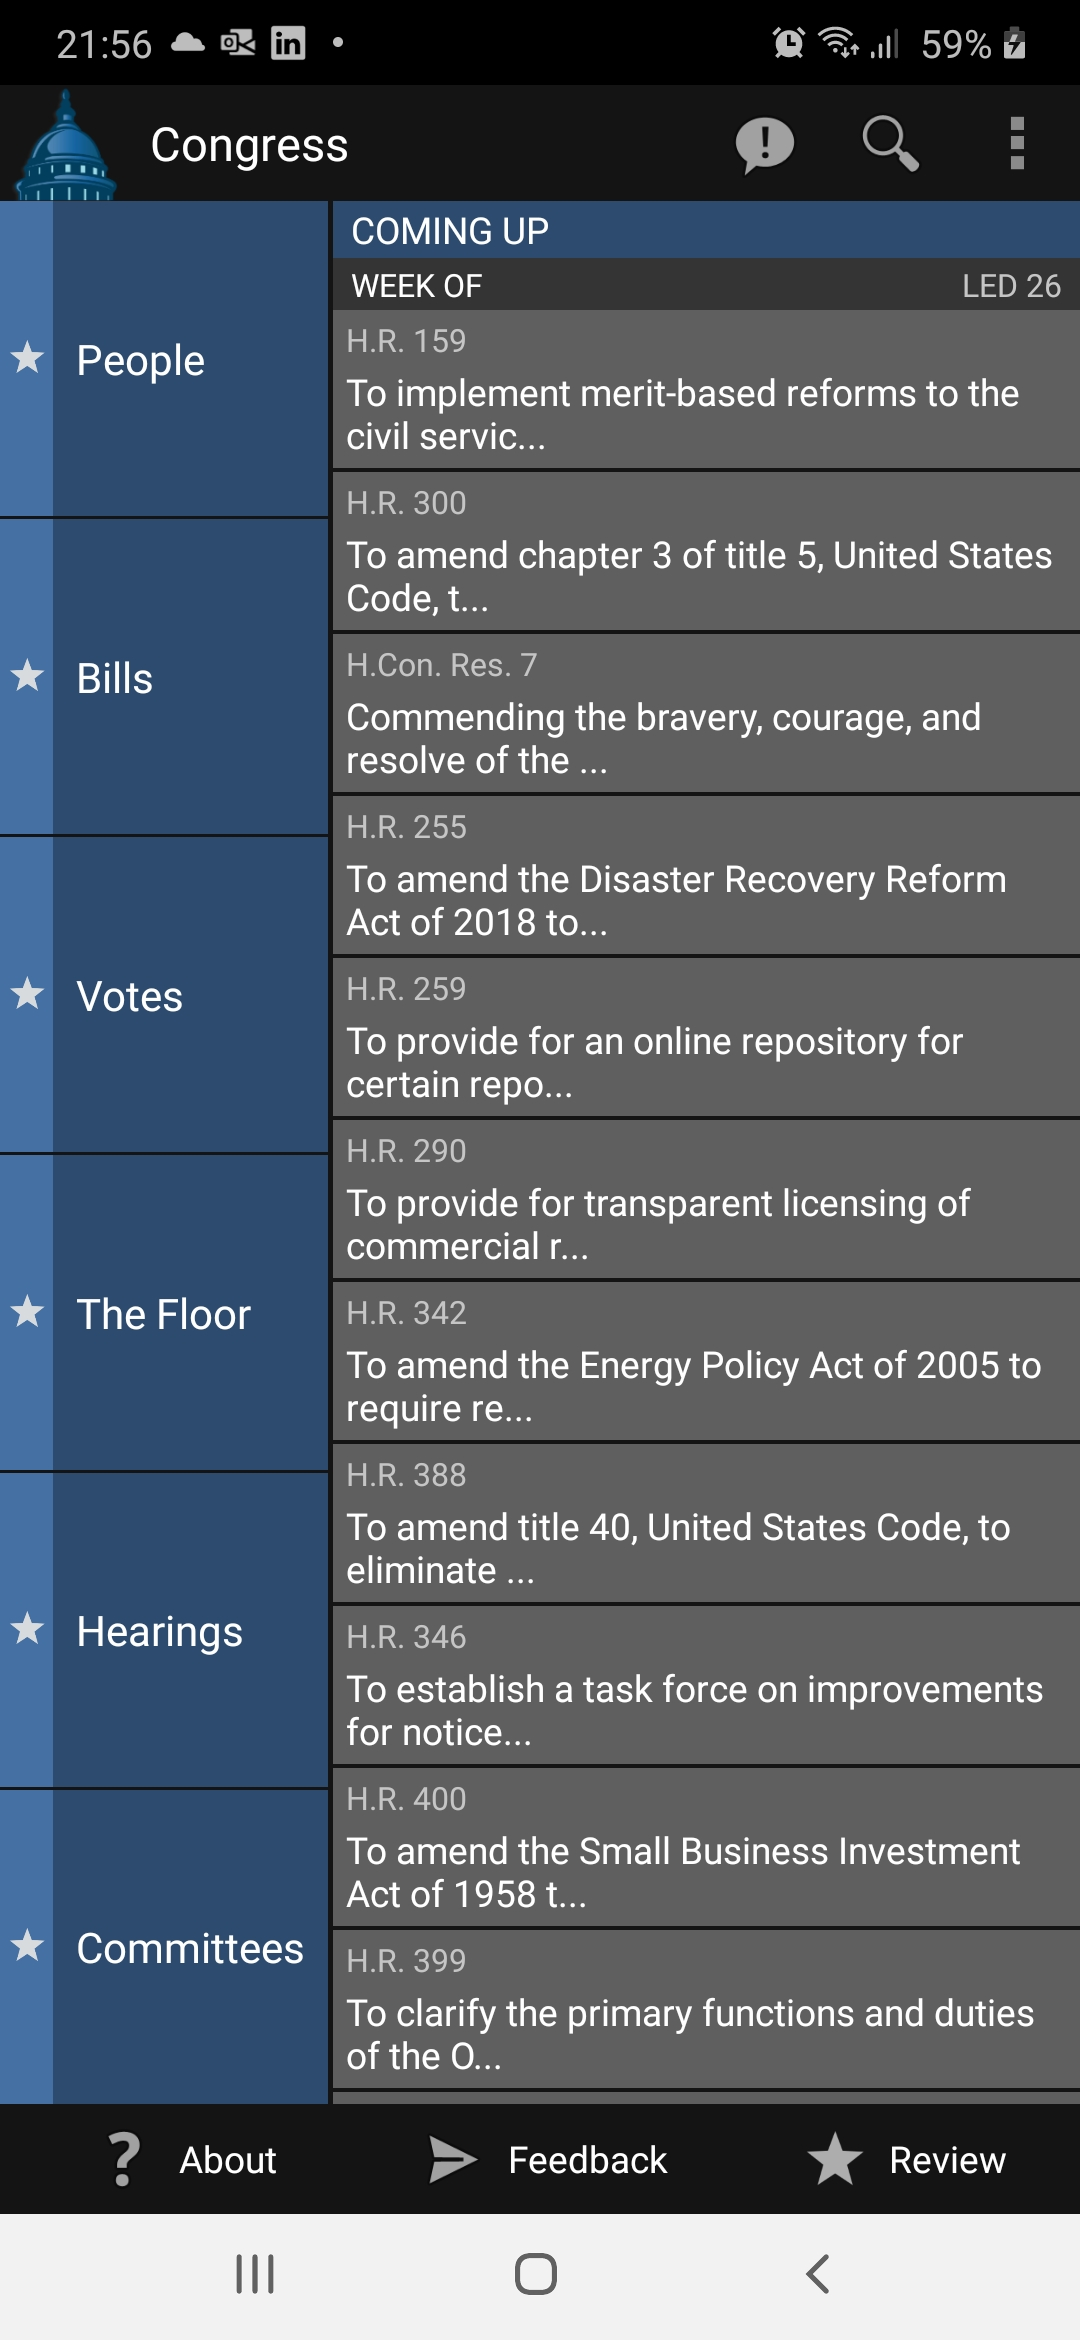
\includegraphics[width=0.4\linewidth]{congress_1}
	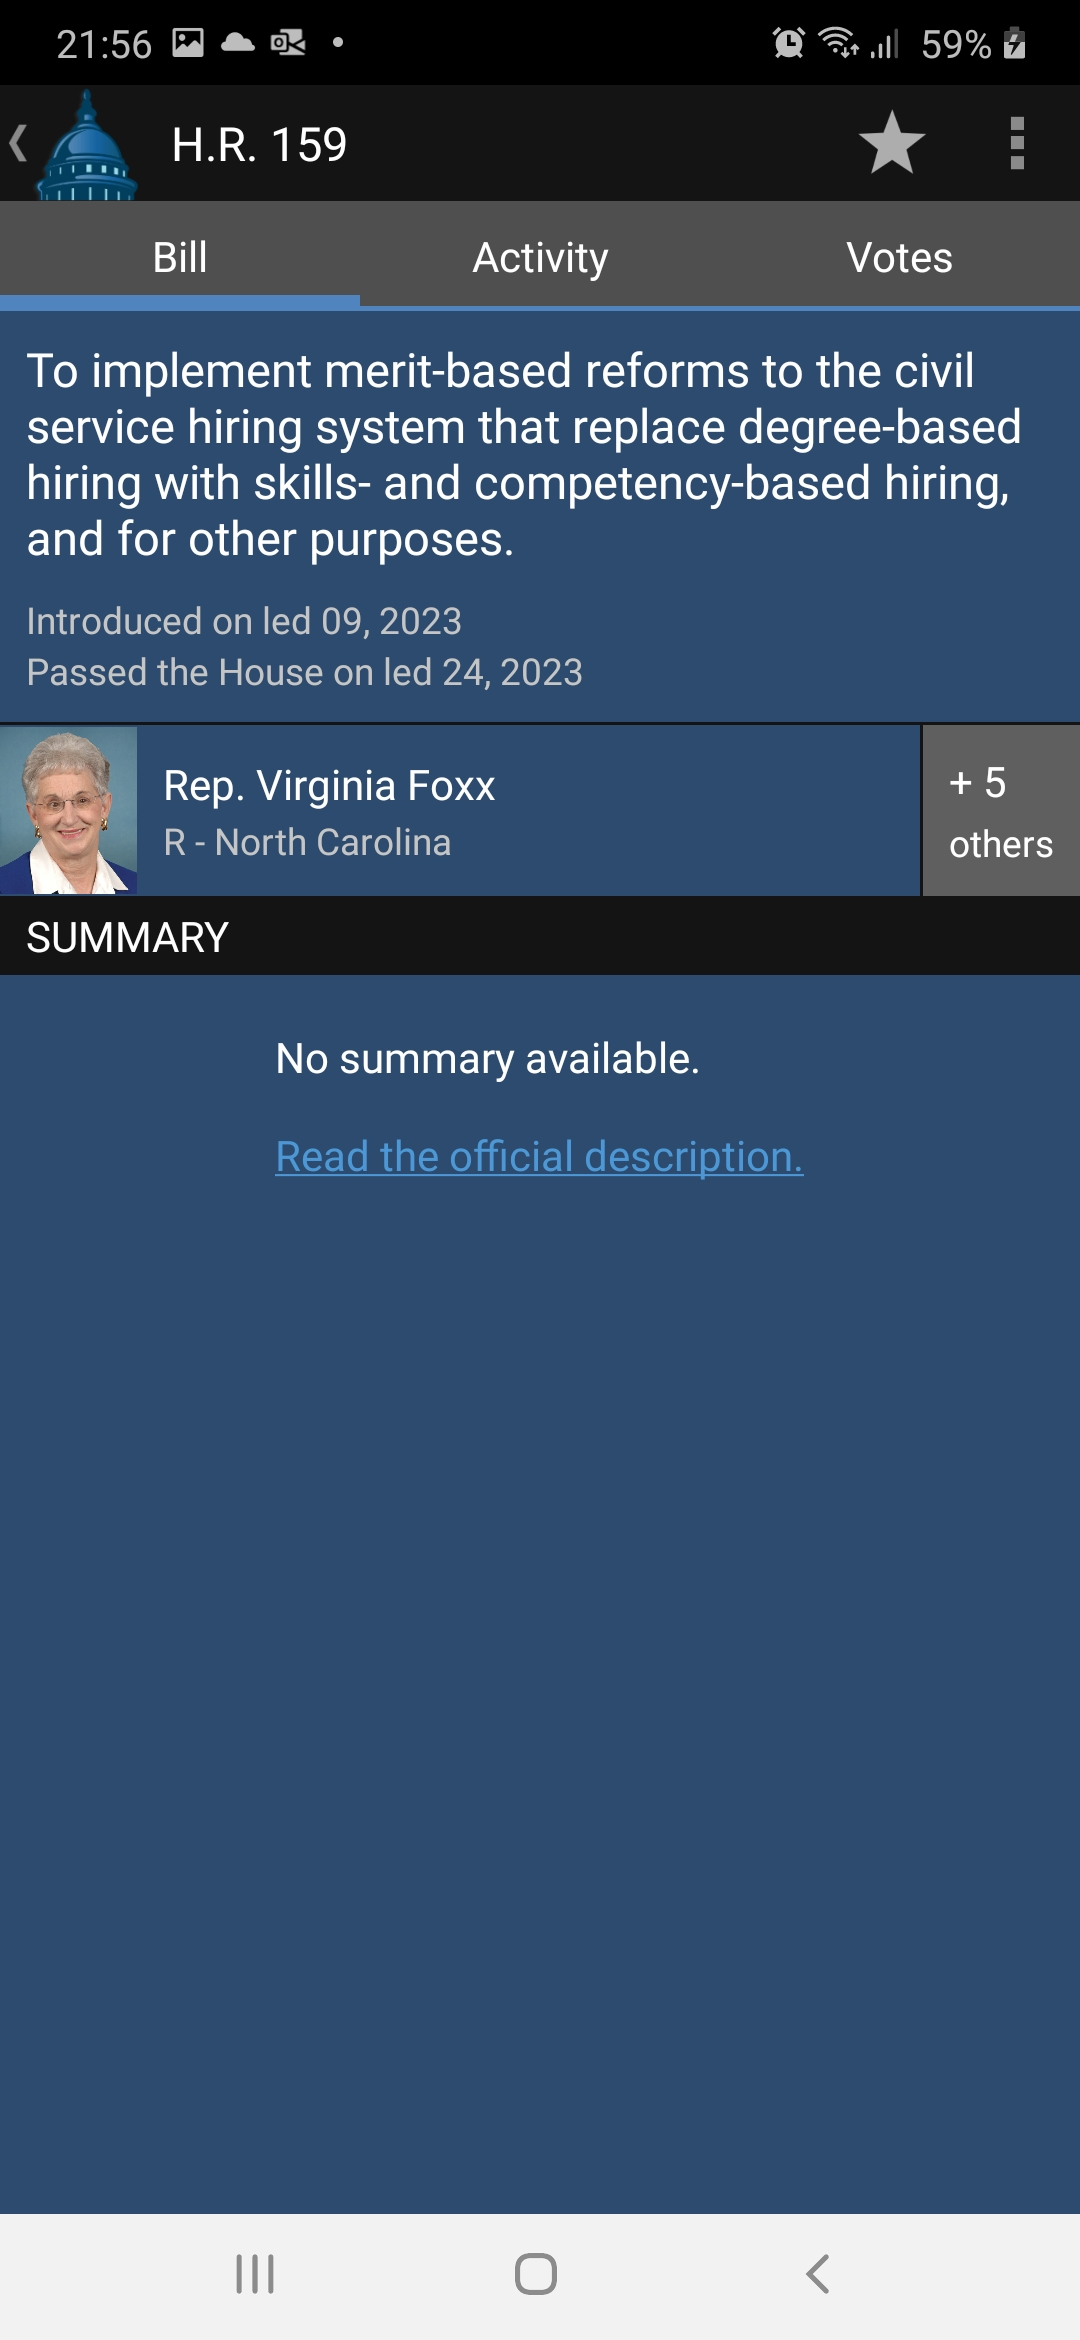
\includegraphics[width=0.4\linewidth]{congress_2}
	
	\caption{Android aplikace politiscope}
	\label{fig:politoscope}
\end{figure}

\subsection{Zhodnocení}
Můj první dojem z této aplikace je to, že je velmi propracovaná z hlediska různorodosti informací, které poskytuje. Přitom díky dobře navrženému uživatelskému rozhraní nepůsobí nepřehledně. Naopak působí velmi intuitivně. Z menu se dostaneme na hlavní obrazovky, které jsou dále rozděleny na taby. U návrhů můžeme snadno vidět výsledek, jak kdo hlasoval, proces schvalování návrhu a aktuální stav. Politici můžeme snadno vyhledat podle klíčových slov, státu a příslušnosti ve Sněmovně nebo Senátu. Politikz a návrhy zákonu můžeme sledovat a nastavit si notifikaci, takže budeme vždy notifikovani o nových změnách.

